\documentclass{article}
\usepackage{iclr2027_conference,times}
\usepackage{amsmath,amssymb,amsthm,graphicx,booktabs,microtype,xcolor}
\usepackage[utf8]{inputenc}
\usepackage{url}
\usepackage{hyperref}
\usepackage{multirow}
\usepackage{float}
\usepackage{tikz}
\usetikzlibrary{positioning,arrows.meta,fit,calc}

\newtheorem{proposition}{Proposition}
\newcommand{\trd}{\textsc{TRD}}
\newcommand{\wrapop}{\operatorname{wrap}}

\title{Native Generation of Tileable Pixel-Art Textures \\
from a Material Name and a Target Colour}

% Authors are hidden unless \iclrfinalcopy is set (ICLR double-blind).
\author{Jingming Zhang, Yi Qi Lim \& Yun Yi Lu Feng \\
Fudan University \\
\texttt{\{jingmingzhang, yiqilim, yunyilufeng\}@fudan.edu.cn} \\
\And
Fei Zhang \\
University of Waterloo \\
\texttt{fei.zhang@uwaterloo.ca}
}

%\iclrfinalcopy % Uncomment for camera-ready only; submissions must stay anonymous

\begin{document}

\maketitle

\begin{abstract}
Game and mod textures are authored natively at tiny canvases: a $16\times16$ tile is not a downscaled photograph but a grid in which every pixel is a design decision, the palette holds at most a handful of slots, and the tile must stay continuous across its own wrap boundary because it is used tiled. We study the task of painting a solid-colour region of an image with a tileable pixel-art texture given only a material name and the region's colour, and we generate it natively at the target resolution rather than rendering large and downsampling. Our model decodes palette-index and luminance-rank tokens in parallel, keeps tileability by construction through a toroidal relative attention bias that adds no parameters, and conditions on palettes retrieved from a memory of artist palettes. Against render-and-downsample pipelines, a same-data pixel-space diffusion baseline, a published score-distillation pixel-art method, and direct retrieval of artist tiles, our $16\times16$ outputs are preferred by a de-biased pairwise judge in the majority of head-to-head comparisons, while costing seconds instead of GPU-hours. Measured end to end, a tile takes $0.51$\,s, $28\times$ faster than the strongest render pipeline and four orders of magnitude faster than score distillation. Getting these comparisons to mean anything required repairing the rulers: we show that render-and-downsample baselines collect a structural gain purely from a larger canvas, that a widely used tiling score awards a perfect value to a flat fill, and that a pairwise judge's resolvable-rate floor is far below chance.
\end{abstract}

\noindent\textbf{Keywords:}
pixel art generation, tileable texture synthesis, masked generative transformer, retrieval-augmented generation, color-conditioned image generation, relative position bias, evaluation of generative models.

\noindent\textbf{Primary Area:}
generative models.

% =====================================================================
\section{Introduction}
\label{sec:intro}

A large share of the textures in voxel games, their mods and many 2D engines
are drawn at $16\times16$. A modder who adds a new block --- ``mossy
cobblestone'', ``birch planks'', ``copper ore'' --- needs a tile that reads as
that material, that fits the colour scheme of the object it is painted on, and
that can be repeated across a wall without a visible seam --- and, iterating
over dozens of blocks, needs it at interactive speed. We study exactly
this task: given an image with a solid-colour region, a material name and the
region's colour, paint the region with a tileable pixel-art texture at
$16\times16$ (and, secondarily, $24\times24$ and $32\times32$).

The obvious route is to render large and shrink. A $1024$px SDXL~\citep{podell2024sdxl}
brick wall is structurally sound, yet every kernel we tried turns it to mush
at $16\times16$: the render packs about $25$ structural units into $16$ cells,
where pixel artists place about three. Cropping the render to its dominant
period repairs this (our baseline B2) but inherits the generator's colours,
seams and cost: every $16$px tile pays for several megapixel renders.
Score distillation~\citep{binninger2024sdpixl} optimises the small image
directly, at hours per tile.

We instead \emph{generate natively}. A pixel-art tile is a small grid of
indices into a palette of at most sixteen colours, so we model it as such: a
masked generative transformer~\citep{chang2022maskgit} that decodes two
discrete token streams in parallel --- sixteen palette slots and an $N\times N$
grid of luminance ranks --- under a text condition, a colour condition and a
palette retrieved from a memory of artist palettes. The transformer has no
absolute positions at all; its only spatial signal is a relative attention
bias defined on the torus, so the network is exactly equivariant to cyclic
shifts and has no notion of where the tile's boundary lies. We call the model
\trd{} (Toroidal Rank Decoding). Native generation is also what makes it
fast: $272$ tokens instead of a megapixel render, half a second per tile.
The recipe is not specific to game textures: the palette--rank representation
fits any palette-indexed image (sprites, icons, tile maps) and the toroidal
bias any periodic one (textile and wallpaper patterns, terrain tiles).

Evaluation at this scale needs care. There is no unique right answer: independent artists drawing the same material agree on
$9.8\%$ of cells against $8.6\%$ expected by chance. Distribution metrics
reward the method that returns artist originals verbatim; a common tiling score
gives a perfect value to a flat fill; and a pairwise VLM judge has to be
validated against a human conclusion before it can be trusted. We
therefore report every comparison with its noise floor, its judge
resolvable-rate floor and a family-level confidence interval, and we call a
comparison a win only when it survives those checks.

\paragraph{Contributions.}
\begin{itemize}
\item \textbf{Task and method.} We formulate region-conditioned pixel-art
  texture generation from a material name and a target colour, and propose
  \trd{}: dual-stream discrete decoding of palette indices and luminance ranks,
  a parameter-light toroidal relative attention bias that makes the model
  cyclic-shift equivariant, and retrieval-augmented palette conditioning
  (\S\ref{sec:method}).
\item \textbf{Results.} On $272$ held-out materials drawn by unseen artists,
  \trd{} has the best KID and FID of all generative methods at $16$px and is
  preferred by a validated, de-biased judge over a same-data pixel diffusion
  model ($63.0\%$), over artist-tile retrieval ($58.9\%$), over SD-$\pi$XL
  ($11/12$) and, on the region-colouring task, over the strongest
  render-and-downsample pipeline ($60.3\%$) (\S\ref{sec:experiments}).
\item \textbf{Efficiency.} A reranked \trd{} tile takes $0.51$\,s end to end
  on one A100, $28\times$ faster than the strongest pipeline and about
  $30{,}000\times$ faster than SD-$\pi$XL (Table~\ref{tab:speed}).
\item \textbf{Measurement.} To make those comparisons meaningful we repair
  three rulers: we show that render-and-downsample baselines collect a
  structural gain purely from a larger canvas, that the raw tiling score
  awards a perfect value to a flat fill, and that the judge's resolvable-rate
  floor on identical pairs is $17.8\%$, far below chance
  (\S\ref{sec:protocol}). Parameter-matched ablations show that both the
  periodic bias and the palette memory are load-bearing: removing either
  roughly triples KID (\S\ref{sec:ablation}).
\end{itemize}

\begin{figure}[t]
\centering
\resizebox{\linewidth}{!}{%
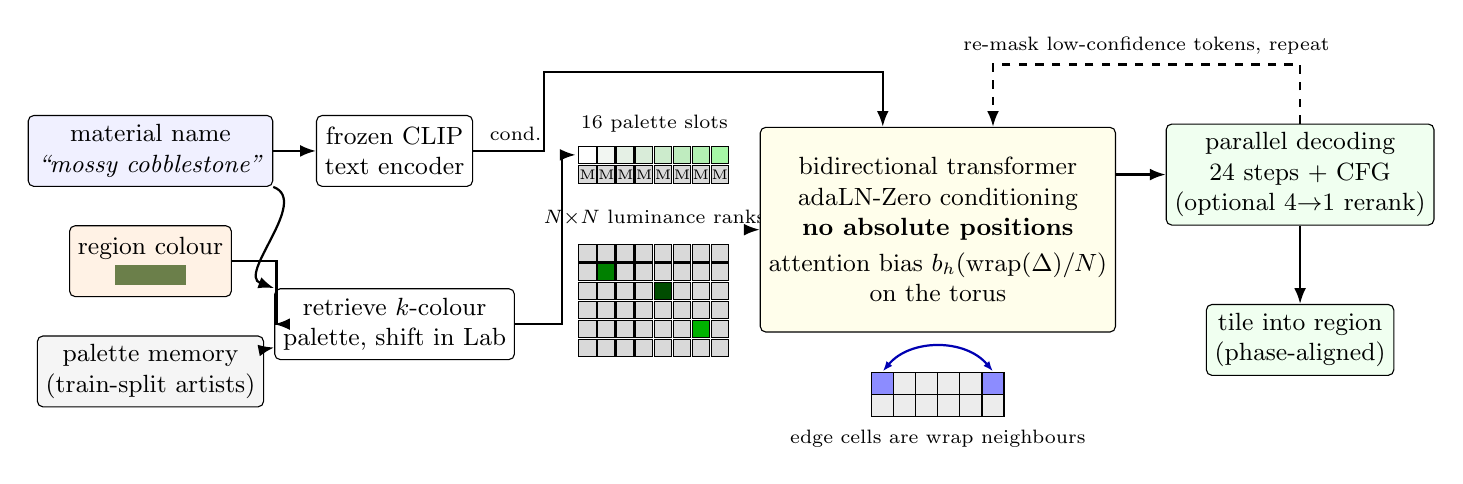
\begin{tikzpicture}[
  font=\small,
  box/.style={draw, rounded corners=2pt, align=center, minimum height=0.9cm, inner sep=3pt},
  tok/.style={draw, minimum size=0.22cm, inner sep=0pt},
  arr/.style={-{Latex[length=2mm]}, thick}]
  % inputs
  \node[box, fill=blue!6] (name) at (0,1.2) {material name\\\textit{``mossy cobblestone''}};
  \node[box, fill=orange!10] (col) at (0,-0.2) {region colour\\\textcolor[HTML]{6B7F4A}{\rule{0.9cm}{0.25cm}}};
  \node[box, fill=gray!8] (mem) at (0,-1.6) {palette memory\\(train-split artists)};
  % encoders
  \node[box] (clip) at (3.1,1.2) {frozen CLIP\\text encoder};
  \node[box] (ret) at (3.1,-1.0) {retrieve $k$-colour\\palette, shift in Lab};
  % tokens
  \node[align=center] (paltxt) at (6.4,1.55) {\scriptsize 16 palette slots};
  \foreach \i in {0,...,7} {\node[tok, fill=green!\the\numexpr 20+10*\i\relax!black!\the\numexpr 5*\i\relax] at (5.55+0.24*\i,1.15) {};}
  \foreach \i in {0,...,7} {\node[tok, fill=gray!30] at (5.55+0.24*\i,0.9) {\tiny M};}
  \node[align=center] (gridtxt) at (6.4,0.35) {\scriptsize $N{\times}N$ luminance ranks};
  \foreach \x in {0,...,7} {\foreach \y in {0,...,5} {\node[tok, fill=gray!30] at (5.55+0.24*\x,-0.1-0.24*\y) {};}}
  \node[tok, fill=green!50!black] at (5.79,-0.34) {};
  \node[tok, fill=green!30!black] at (6.51,-0.58) {};
  \node[tok, fill=green!70!black] at (6.99,-1.06) {};
  % transformer
  \node[box, fill=yellow!8, minimum width=2.9cm, minimum height=2.6cm] (tf) at (10.0,0.2)
     {bidirectional transformer\\ adaLN-Zero conditioning\\ \textbf{no absolute positions}\\[2pt]
      attention bias $b_h(\wrapop(\Delta)/N)$\\ on the torus};
  % wrap-around neighbourhood: left and right edge cells are adjacent
  \foreach \x in {0,...,5} {\foreach \y in {0,1} {\node[tok, minimum size=0.28cm, fill=gray!15] at (9.3+0.28*\x,-1.75-0.28*\y) {};}}
  \node[tok, minimum size=0.28cm, fill=blue!45] at (9.3,-1.75) {};
  \node[tok, minimum size=0.28cm, fill=blue!45] at (10.7,-1.75) {};
  \draw[{Latex[length=1.3mm]}-{Latex[length=1.3mm]}, blue!70!black, thick] (9.3,-1.6) to[out=50,in=130] (10.7,-1.6);
  \node[font=\scriptsize, align=center] at (10.0,-2.45) {edge cells are wrap neighbours};
  % output
  \node[box, fill=green!6] (out) at (14.6,0.9) {parallel decoding\\24 steps + CFG\\(optional 4$\to$1 rerank)};
  \node[box, fill=green!6] (paint) at (14.6,-1.2) {tile into region\\(phase-aligned)};
  % arrows
  \draw[arr] (name) -- (clip);
  \draw[arr] (col) -- ++(1.6,0) |- (ret);
  \draw[arr] (mem) -- (ret);
  \draw[arr] (name.south east) to[out=-20,in=160] (ret.north west);
  \draw[arr] (ret.east) -- ++(0.6,0) |- (5.4,1.15);
  \draw[arr] (clip.east) -- ++(0.9,0) node[above, pos=0.6, font=\scriptsize]{cond.} -- ++(0,1.0) -| ([xshift=-7mm]tf.north);
  \draw[arr] (7.55,0.2) -- (tf.west);
  \draw[arr] (tf.east |- out.west) -- (out.west);
  \draw[arr] (out) -- (paint);
  \draw[arr, dashed] (out.north) -- ++(0,0.75) -| node[above, pos=0.25, font=\scriptsize]{re-mask low-confidence tokens, repeat} ([xshift=7mm]tf.north);
\end{tikzpicture}}
\caption{\trd{} at a glance. A material name and a region colour are turned
into a text condition and a retrieved artist palette. Palette slots and a grid
of luminance ranks are decoded jointly by iterative parallel unmasking. The
transformer's only spatial signal is a relative bias on wrapped offsets, so
cells on opposite edges of the tile are treated exactly as interior
neighbours.}
\label{fig:overview}
\end{figure}

% =====================================================================
\section{Related Work}
\label{sec:related}

Three research lines meet in this task and, as far as we can tell, rarely cite
one another.

\paragraph{Pixel-art generation and pixelization.} SD-$\pi$XL~\citep{binninger2024sdpixl}
produces palette-constrained low-resolution images from a text prompt by score
distillation~\citep{poole2023dreamfusion} from a latent diffusion
model~\citep{rombach2022ldm}; its first listed contribution is that it works
at any resolution. It optimises each image separately, has no region channel
and no notion of wrap-around. Pixelization methods convert an existing
high-resolution image: \citet{gerstner2012pixelated} jointly optimise a palette
and a superpixel grid, \citet{wu2022pixelization} learn aliasing-aware,
cell-controllable pixelization, and content-adaptive or perceptual
downscaling~\citep{kopf2013downscaling,oztireli2015downscaling} optimises the
kernel for a given scale factor. Classical palette
quantization~\citep{heckbert1982quantization} and
dithering~\citep{floyd1976} are post-processing steps. All of these take the
high-resolution image as given; for generated sources the binding constraint
is how many structural units the source contains, which no kernel can change.

\paragraph{Tileable texture synthesis.} Non-parametric
synthesis~\citep{efros1999texture,efros2001quilting} and neural
statistics~\citep{gatys2015texture} synthesise textures from exemplars;
procedural noise~\citep{perlin1985,worley1996} is tileable by construction but
not text-conditioned. Diffusion-based methods enforce tileability at sampling
time: TileGen~\citep{zhou2022tilegen} and ControlMat~\citep{vecchio2024controlmat}
use circular padding or rolled noise for materials, and Tiled
Diffusion~\citep{madar2025tiled} generalises seam-consistent sampling across
tiles. TexTile~\citep{rodriguezpardo2024textile} proposes a learned
tileability metric. These works operate at $\geq256$px on photographic
materials; our same-data diffusion baseline B7 uses the circular-padding
recipe. At $16$px, our toroidal bias both gives exact shift equivariance and
is what makes quality possible (\S\ref{sec:ablation}).

\paragraph{Colour-conditioned and retrieval-augmented generation.}
ColorPeel~\citep{butt2024colorpeel} learns colour prompts that disentangle
colour from shape, and ControlNet-style adapters~\citep{zhang2023controlnet}
inject spatial or palette guidance into a frozen model. Retrieval-augmented
diffusion~\citep{blattmann2022rdm,sheynin2023knndiffusion,chen2023reimagen}
conditions generation on nearest neighbours from an external memory. We
retrieve only palettes, not images, and feed them as known tokens, so the
structure is always generated.

\paragraph{Masked and discrete generative models.} MaskGIT~\citep{chang2022maskgit}
and Muse~\citep{chang2023muse} decode VQ tokens~\citep{vandenoord2017vqvae} in
parallel with a cosine masking schedule, a special case of absorbing-state
discrete diffusion~\citep{austin2021d3pm}; Token-Critic~\citep{lezama2022tokencritic},
MAGE~\citep{li2023mage} and MaskBit~\citep{weber2024maskbit} refine the
sampler and the tokenizer. Pixel art needs no learned tokenizer: its native
representation is already discrete. Relative position
biases~\citep{shaw2018relative,raffel2020t5,liu2021swin,wu2021irpe} are
standard in vision transformers; we restrict ours to the torus and study
whether its periodic form is what matters, in the spirit of equivariant
architectures~\citep{cohen2016gcnn}.

\paragraph{Judging generative models.} Pairwise VLM judges are
common~\citep{zheng2023mtbench}, with documented positional
bias~\citep{wang2024fair}, order-swap inconsistency~\citep{webdevjudge2025}
and poor absolute scoring~\citep{kumar2026rankscore}; distribution
metrics~\citep{heusel2017fid,binkowski2018kid,stein2023exposing,oquab2024dinov2}
were calibrated on natural images at $\geq224$px.

% =====================================================================
\section{Why a 16$\times$16 Tile Is Not a Small Image}
\label{sec:task}

\paragraph{Data.} We collected every texture pack with a clean licence and an
explicit resolution tag from the Luanti (Minetest) ContentDB: $105$ packs were
scanned, packs whose licence forbids training were excluded, and
Minecraft-derived packs were excluded entirely. Because the engine uses a
shared file name for each block across packs (e.g.\ \texttt{default\_wood.png}),
file names are free, artist-aligned material labels. After dropping tiles with
fewer than three native colours the corpus has $5{,}979$ tiles from $76$ packs
covering $521$ materials ($4{,}951$ at $16$px, $679$ at $32$px, $349$ at
$64$px). The split is \emph{by pack}: $57$ packs for training ($4{,}248$
tiles), $7$ for validation ($460$) and $12$ for testing ($1{,}271$). Because a
pack has one visual style, a pack-level split means every test tile is drawn by
an artist the model has never seen, while $448$ of the $450$ test materials
occur in training under other artists.

\paragraph{Every pixel is a decision.} In the $16$px subset the median native
colour count is $16$ and $2{,}172$ of $4{,}951$ tiles use a full sixteen-slot
palette; there is no anti-aliasing, and edges are hard. Dithering, often cited
as the characteristic difficulty, is rare: a $50\%$ checkerboard signature
appears \emph{less} often than under a within-tile shuffle null, and tiles are
dominated by coherent stripes and blocks.

\paragraph{There is no right answer.} Because a tile is a grid of palette
indices, agreement between two artists who drew the same material is exactly
computable. Over $50{,}753$ same-material artist pairs, per-cell agreement is
$0.098$ against $0.086$ under a paired shuffle null that preserves each tile's
own marginal. A per-pixel reconstruction target is therefore meaningless for
this task, which is why we model a distribution and why evaluation needs the
care of \S\ref{sec:protocol}.

\paragraph{Why not render and shrink?} Artist tiles hold a median of $3.2$
structural units at both $16$ and $32$px; a $1024$px SDXL render holds about
$25$, so it must be cropped before any kernel can help
(Figure~\ref{fig:b2}, appendix).

% =====================================================================
\section{Method}
\label{sec:method}

\subsection{A discrete, colour-factored representation}
\label{sec:repr}

Each training tile $x\in\{\text{RGB}\}^{N\times N}$ is quantised to at most
$K=16$ colours by median cut and \emph{canonicalised}: the $k\le K$ colours it
uses are sorted by luminance, the grid stores each pixel's luminance rank
$r_{ij}\in\{0,\dots,k-1\}$, and the palette stores the colours
$(c_0,\dots,c_{k-1})$ in the same order as codes in a $512$-entry colour
codebook. The mapping is exactly invertible. A tile is thus the token sequence
\begin{equation}
  s = \big[\,c_0,\dots,c_{k-1},\underbrace{\texttt{PAD},\dots}_{K-k}\;\big|\; r_{11},\dots,r_{NN}\,\big],
  \qquad |s| = K + N^2,
\end{equation}
with $|s|=272$ at $16$px. The factorisation separates \emph{structure} (which
cell is darker than which) from \emph{colour} (what the levels are), which is
what lets the palette be retrieved or shifted to a user's colour without
touching the structure, and it matches how pixel artists work: a ramp of
shades, placed by hand. Because a rank token means different things for
different $k$ (rank $2$ is the brightest level of a $3$-colour tile and a dark
one of a $16$-colour tile), each grid token additionally receives an embedding
of its normalised level $\operatorname{round}(15\,r/(k-1))$, and logits for
ranks $\ge k$ are masked.

\subsection{Toroidal relative attention bias}
\label{sec:bias}

The backbone is a bidirectional transformer~\citep{vaswani2017attention} of
$12$ blocks, width $384$ and $6$ heads. It has \emph{no absolute position
embedding}. Instead every block adds to the attention logits a bias that
depends only on the offset between two grid cells taken on the torus. For
cells at $p_i,p_j\in\{0,\dots,N-1\}^2$ let
$u = \wrapop\!\big((p_i-p_j)/N\big)\in[-\tfrac12,\tfrac12)^2$ with
$\wrapop(t)=((t+\tfrac12)\bmod 1)-\tfrac12$ applied per axis. The bias is
\begin{equation}
  b_h(i,j) = \mathrm{MLP}_h\big(\phi(u)\big),\qquad
  \phi(u) = \big[\sin 2\pi f u_y,\ \cos 2\pi f u_y,\ \sin 2\pi f u_x,\ \cos 2\pi f u_x\big]_{f=1}^{F},
  \label{eq:bias}
\end{equation}
with $F=8$ harmonics, which suffices to represent any function on a $16$-cell
circle~\citep{tancik2020fourier}. Palette tokens have no position; the
palette--palette block of the bias is a learned $K\times K$ table per head and
the palette--grid blocks are learned scalars. One bias module is shared by all
blocks; with a $128$-unit hidden layer it has about $6.5$k parameters,
fewer than a single learned absolute embedding of the $16\times16$ grid
($98$k). Its toroidal form costs nothing over an ordinary relative bias of the
same shape --- the wrap is applied to the input, not learned.

\begin{proposition}
Let $T_\delta$ cyclically shift the grid tokens of $s$ by $\delta\in\mathbb{Z}_N^2$
and leave palette tokens fixed. If the network uses no absolute positions and
its attention bias between grid tokens depends only on $\wrapop((p_i-p_j)/N)$,
then its logits satisfy $f(T_\delta s)=T_\delta f(s)$ for all $\delta$.
\end{proposition}
\emph{Proof sketch.} Token-wise operations (embeddings, MLPs, adaLN) commute
with any permutation of tokens. Attention logits $q_i^\top k_j+b(i,j)$ are
permuted by $T_\delta$ because $\wrapop((p_i+\delta-p_j-\delta)/N)=\wrapop((p_i-p_j)/N)$,
and the palette--grid terms are position-independent. \qed
The trained model satisfies this to float32 precision: over five shifts at
$16$ and $32$px, grid logits of the shifted input differ from the shifted
logits by at most $1.1\times10^{-5}$ (logit s.d.\ $1.1$), whereas the
non-periodic and wrong-period variants of \S\ref{sec:ablation} deviate by
$1.4$--$5.1$.

Because masked decoding samples positions with i.i.d.\ Gumbel perturbations,
the sampling distribution inherits the invariance: the model assigns the same
probability to a tile and to every cyclic shift of it, so the tile boundary is
not a privileged location. This is the precise sense in which
tileability is built in. Whether the \emph{periodic} form of the bias is what
makes the model work is a separate, empirical question, which we test with
parameter-matched replacements in \S\ref{sec:ablation}.

\subsection{Conditioning and retrieval-augmented palettes}
\label{sec:cond}

\paragraph{Text, colour and palette size.} The material name is embedded as
``pixel art texture of \{name\}'' by a frozen CLIP text
encoder~\citep{radford2021clip}, which makes the vocabulary open. The region
colour enters as $[r,g,b,1]$ (all zeros when dropped; the flag distinguishes
``no colour'' from black) and the palette size $k$ as a learned embedding. The
three are summed into one vector that modulates every block through
adaLN-Zero~\citep{peebles2023dit}. During training the text is dropped for $10\%$ of
examples to enable classifier-free guidance~\citep{ho2022cfg}, and the colour
is dropped for half of them.

\paragraph{Palette memory.} A $512$-way palette head trained on a few
thousand tiles learns the marginal of colours but not the ramps artists
actually use. We therefore keep a memory
of every training-split palette with its material, CLIP text embedding, colour
count and mean colour, and at inference retrieve instead of generate. For a
query name we take the $n_\text{name}$ nearest training materials in CLIP text
space, rank their tiles by cross-modal CLIP similarity between the query text
and the tile image, optionally restrict to palettes whose mean colour is close
to the target in Lab ($\Delta E$), and sample one of the top $5$. The
retrieved palette is shifted in Lab so its mean lands on the region colour,
and fed to \trd{} as \emph{known} palette tokens; only the grid is generated.
The memory contains palettes, not images, and is built from training packs
only, so no test artist's work can be retrieved.

\paragraph{Structural exemplars.} Four same-material training tiles by other
artists can be appended as position-free, never-predicted tokens; they are
optional, and the model is robust to their removal (\S\ref{sec:ablation}).

\subsection{Training and parallel decoding}
\label{sec:decode}

\paragraph{Objective.} We train with the MaskGIT objective: a mask ratio
$\gamma=\cos(\tfrac{\pi}{2}u)$, $u\sim\mathcal U(0,1)$, is drawn per example,
palette and grid tokens are masked independently at that ratio, and the loss
is cross-entropy on masked tokens of both streams. Every example is
cyclically shifted by a uniformly random offset (all $N^2$ phases are valid
samples of a tileable texture) and horizontally flipped with probability
$\tfrac12$. We use AdamW with learning rate $3\times10^{-4}$, weight decay
$0.05$, $1{,}000$ warm-up steps and batch $256$; the $16$px model is trained
for $20$k steps, and a second checkpoint trained jointly on $16$ and $32$px is
used for the $24$ and $32$px results. At roughly $0.3$\,s per step on one
A100, a model trains in under two GPU-hours.

\paragraph{Decoding.} Sampling starts from a fully masked grid (and the
retrieved palette) and runs $24$ steps. At each step all masked tokens are
sampled in parallel, and the least confident are re-masked according to the
cosine schedule, with Gumbel noise on the confidences annealed to zero
(choice temperature $20$) and classifier-free guidance of weight $1.5$. As an
optional last stage (``+rr'') we draw four samples and keep the one whose
CLIP ViT-B/16 image embedding best matches the prompt; evaluation uses a
different CLIP (ViT-B/32), so the reranker does not grade its own homework.
The tile is then written into the region with its phase aligned to the
region's bounding box.

\paragraph{Speed.} Table~\ref{tab:speed} times the exact test-time
configurations on one A100. Existing routes are slow for structural reasons:
a render pipeline runs a $2.6$B-parameter U-Net $28$ times on a $128^2$
latent per render, four renders per tile, then discards over $99.9\%$ of the
pixels; score distillation back-propagates through that network at each of
$10$k steps per tile. \trd{} removes each cost by construction: it generates
at the target resolution ($272$ tokens), its discrete tokens \emph{are} the
tile (no latent decoder), decoding is parallel ($24$ steps), palettes are
looked up, and the toroidal bias needs no crop, period search or seam repair.

\begin{table}[t]
\caption{Cost per delivered $16$px tile on one A100 (wall clock, exact
test-time settings). \trd{}+rr: all $272$ test materials end to end,
\emph{including} model loading ($138.6$\,s total). B2: per material,
\emph{excluding} model loading. SD-$\pi$XL: median over its test subset.}
\label{tab:speed}
\centering
\small
\begin{tabular}{@{}lccccr@{}}
\toprule
Method & Params & Generated at & Sequential steps & Time / tile & Relative \\
\midrule
SD-$\pi$XL (B3) & $2.6$B (SDXL) & $16^2$, optimised & $10$k optimisation & $4.44$\,h & $\approx31{,}000\times$ \\
B2 render + crop & $2.6$B (SDXL) & $4\times1024^2$ & $4\times28$ denoising & $14.5$\,s & $28\times$ \\
\trd{}+rr (ours) & $33$M & $4\times272$ tokens & $24$ parallel & $\mathbf{0.51}$\,s & $1\times$ \\
\bottomrule
\end{tabular}
\end{table}

% =====================================================================
\section{Evaluation Protocol: Repairing the Rulers}
\label{sec:protocol}

We report the metrics used by the pixel-art and texture literature and, for
each, the evidence a reader needs to know how large a difference has to be.

\paragraph{Distribution and alignment metrics.} KID~\citep{binkowski2018kid}
($\times10^3$), FID~\citep{heusel2017fid} with Inception
features~\citep{szegedy2016inception} and FD-DINOv2~\citep{stein2023exposing}
against the test-split artist tiles, CLIP score~\citep{hessel2021clipscore}
against ``pixel art texture of \{name\}'', and LPIPS~\citep{zhang2018lpips}
diversity between samples of the same prompt. Tiles are enlarged with nearest
neighbour to the network input size, identically for artists and methods.
Two floors calibrate these numbers. Retraining the same recipe with three
seeds moves $16$px KID by at most $1.09$; resampling one checkpoint once per
material moves it by up to $4.76$ ($2.70$ with four samples per material), and
FID, FD and CLIP by $6.0$, $20$ and $0.41$. We only interpret a difference
that exceeds the larger of the two floors.

\paragraph{Ruler 1: a flat fill has a perfect tiling score.} A common tiling
score sums colour differences across the wrap seam of a $3\times3$ tiling. We
ran it on constructed counterexamples. A tile filled with its own mean colour
scores exactly $0.000$, better than every real method (the best, B4, scores
$5.31$) and far better than artist tiles ($19.9$). Blurring or flattening the
border likewise improves the raw score. We therefore report the ratio of
across-seam to interior neighbour differences, whose ideal is $1$: it returns
\emph{undefined} for a flat fill and $0$ for a flattened border, so neither
can win, and deviations on both sides count as failures. Even this ratio is a
property check, not a quality axis: a cyclic shift of the artist tiles changes
their median $|r-1|$ from $0.469$ to $0.234$.

\paragraph{Ruler 2: a larger canvas buys structure for free.} B2 crops its
render to $4.5$ dominant periods before downsampling, independently of the
target size, so at $32$px it shows the same structure with twice the cells.
Asked to compare B2 at $32$px with B2 at $16$px enlarged to the same size, the
judge prefers the former $107/138=78\%$ ($p=5.5\times10^{-11}$, family CI
$[0.69,0.86]$). The render-and-downsample family therefore improves with the
canvas for reasons unrelated to the method, and a curve of win rate against
resolution mixes that gain with the method's quality. We compare methods only
within a resolution and refuse to read the three resolutions as one curve.

\paragraph{Ruler 3: human ground truth, scaled by a certified judge.}
Preference is anchored in human judgement. Four annotators labelled a blind
study of $60$ pairs with sides randomised, resolved to a consensus label,
which reached a clear conclusion (one condition preferred in $49/59=83\%$ of
decided pairs). To extend this human protocol to all $272$ test materials and
every arm, we admit a pairwise VLM judge only if it reproduces the human
conclusion: of three frontier judges, only \texttt{claude-opus-5} did ($73\%$,
$p=0.008$); another, with identical per-item agreement ($66.7\%$), compressed
it to $62\%$ ($p=0.14$), and the third inverted it. The judge is thus a
scaled-up proxy certified against the annotators, not an independent
authority. Each pair is asked in both orders and a
verdict counts only if both orders agree. To measure what this protocol can
resolve, we submit $118$ \emph{empty} pairs --- the same image on both sides.
An ideal judge never resolves them; one that answered at random would resolve
$50\%$. The judge resolves $21/118=17.8\%$, far below chance, whereas real
comparisons are resolved $74$--$78\%$ of the time, so decided verdicts carry
signal. We report wins over decided pairs, a two-sided binomial $p$, and a
\emph{family-level} $95\%$ interval obtained by resampling material families,
which accounts for the fact that related materials (all the ``planks'') are
not independent~\citep{cameron2011cluster}. A comparison is called robust only
if that interval excludes $0.5$.

% =====================================================================
\section{Experiments}
\label{sec:experiments}

\subsection{Setup and baselines}

The formal test set (E\_mat) has $272$ materials with $857$ artist tiles from
the $12$ held-out packs; it was generated once, under a pre-registered
protocol, after all design choices were frozen on the validation packs. Each
baseline blocks one objection.
\textbf{B1} (``just shrink a big model''): SDXL at $1024$px, box downsample,
quantise to $16$ colours.
\textbf{B2} (the industrial answer): our own render pipeline --- best of four
SDXL renders, crop to the detected dominant period, seam-aligned window, then
downsample and quantise (Appendix, Figure~\ref{fig:b2}).
\textbf{B3} (a published pixel-art method): SD-$\pi$XL with its released code,
on $12$ materials, as each tile takes over four hours (Table~\ref{tab:speed}).
\textbf{B4} (``add a pixel-art LoRA''): SDXL with the public
\texttt{pixel-art-xl} LoRA~\citep{hu2022lora}, then B1's downsampling.
\textbf{B5} (``retrieval has the best FID''): an artist tile retrieved from
the training split by prompt co-occurrence.
\textbf{B7} (``native generation is enough'' and ``why not circular
padding''): a $29.9$M-parameter pixel-space diffusion
U-Net~\citep{ronneberger2015unet,ho2020ddpm} trained from scratch on
\emph{our} data with text and colour conditioning, circular padding,
classifier-free guidance, $50$ DDIM steps and $16$-colour quantisation; it
removes the data advantage as an explanation. \trd{} denotes the single-sample
model and \trd{}+rr the four-to-one reranked variant.

\subsection{Main results at 16px}

\begin{table}[t]
\caption{Name-to-texture at $16$px on the held-out test set ($272$ materials,
$857$ artist tiles, unseen artists). KID is $\times10^3$. Seam: median
$|r-1|$ of the seam ratio (ideal $0$, a property check only). B5 returns
artist originals and is listed as a reference, not a generator. Noise floors:
KID $4.76$, FID $6.0$, FD $20$, CLIP $0.41$.}
\label{tab:main}
\centering
\small\setlength{\tabcolsep}{5pt}
\begin{tabular}{@{}lcccccc@{}}
\toprule
Method & KID $\downarrow$ & FID $\downarrow$ & FD-DINOv2 $\downarrow$ & CLIP $\uparrow$ & LPIPS div.\ $\uparrow$ & Seam $|r{-}1|$ \\
\midrule
B1 SDXL + downsample & 52.2 & 85.9 & 206.8 & 34.51 & 0.217 & 0.173 \\
B2 render + crop + downsample & 28.9 & 65.4 & 217.4 & \textbf{35.21} & -- & 0.530 \\
B4 SDXL + pixel-art LoRA & 76.7 & 104.6 & 253.7 & 34.97 & 0.138 & 0.190 \\
B7 same-data pixel diffusion & 10.0 & 45.5 & \textbf{59.3} & 33.17 & \textbf{0.355} & 0.232 \\
\midrule
\trd{} (ours) & \textbf{8.8} & \textbf{43.2} & 82.3 & 34.60 & 0.303 & 0.201 \\
\trd{}+rr (ours) & 9.7 & 44.2 & 77.5 & 35.19 & -- & 0.178 \\
\midrule
\textcolor{gray}{B5 artist retrieval (reference)} & \textcolor{gray}{2.7} & \textcolor{gray}{43.0} & \textcolor{gray}{45.3} & \textcolor{gray}{32.95} & \textcolor{gray}{0.382} & \textcolor{gray}{0.614} \\
\bottomrule
\end{tabular}
\end{table}

\paragraph{Distribution metrics.} Table~\ref{tab:main} shows that \trd{} has
the lowest KID and FID of all generators. Against the SDXL family the margins
are far outside the noise floor: KID drops from $28.9$ (B2) and $52.2$ (B1) to
$8.8$, FID from $65.4$ to $43.2$, and FD-DINOv2 from $217$ to $82$. Reranking
brings CLIP level with B2 ($35.19$ vs $35.21$, well within the $0.41$ floor)
at a KID that is still three times lower. Against B7, trained on the same data,
\trd{} has lower KID ($8.8$ vs $10.0$) and FID ($43.2$ vs $45.5$) and is
clearly better aligned with the material name (CLIP $+1.43$, beyond the
floor); where the metrics split, the judge decides ($63.0\%$, below). The retrieval reference B5 dominates every
distribution metric simply by returning artist originals; the next paragraph
shows that this does not make it better.

\paragraph{Pairwise judgements.} Table~\ref{tab:judge} and
Figure~\ref{fig:forest} report the main $16$px arms (all arms:
App.~\ref{app:res}; samples: App.~\ref{app:qual}).
\trd{} is preferred over the same-data diffusion model B7 in $63.0\%$ of
decided pairs (family CI $[0.54,0.72]$), so the advantage is architectural,
not a matter of data. \trd{}+rr is preferred over artist retrieval B5 in
$58.9\%$ ($[0.50,0.67]$), although B5 has the best KID, FID and FD of any
entry in Table~\ref{tab:main} --- direct evidence on this task that
distribution match and preference diverge. Against SD-$\pi$XL, \trd{} wins
$11/12$ materials ($p=0.0064$). Against the strongest pipeline B2,
\trd{}+rr is preferred in $57.3\%$ of decided pairs ($p=0.047$) --- a native $33$M-parameter generator matching
and edging out a pipeline built on a $2.6$B-parameter diffusion model with
best-of-four selection and a hand-tuned period crop.

\begin{table}[t]
\caption{De-biased pairwise judge at $16$px (\texttt{claude-opus-5}, both
orders, inconsistent pairs discarded). ``Family CI'' resamples material
families; \textbf{robust} = excludes $0.5$. Floor on identical pairs:
$17.8\%$ resolved. Colour task: region colour given to every method; all
baselines receive the same Lab residual recolouring.}
\label{tab:judge}
\centering
\small\setlength{\tabcolsep}{4.5pt}
\begin{tabular}{@{}llcccc@{}}
\toprule
Task & Comparison (first wins) & Wins / decided & Rate & $p$ & Family 95\% CI \\
\midrule
\multirow{4}{*}{Name$\to$texture}
 & \trd{} vs B7 & 131 / 208 & 63.0\% & $2.2\times10^{-4}$ & \textbf{[0.540, 0.719]} \\
 & \trd{}+rr vs B5 & 119 / 202 & 58.9\% & $0.014$ & \textbf{[0.502, 0.668]} \\
 & \trd{} vs B3 (SD-$\pi$XL, 12 mat.) & 11 / 12 & 91.7\% & $0.0064$ & n/a \\
 & \trd{}+rr vs B2 & 114 / 199 & 57.3\% & $0.047$ & [0.500, 0.641] \\
\midrule
\multirow{3}{*}{Region colour}
 & \trd{} vs B2 & 114 / 189 & 60.3\% & $0.0056$ & \textbf{[0.525, 0.680]} \\
 & \trd{} vs B7 & 117 / 193 & 60.6\% & $0.0039$ & \textbf{[0.524, 0.674]} \\
 & \trd{} vs B5 (+recolour) & 111 / 208 & 53.4\% & $0.37$ & [0.434, 0.627] \\
\bottomrule
\end{tabular}
\end{table}

\begin{figure}[t]
\centering
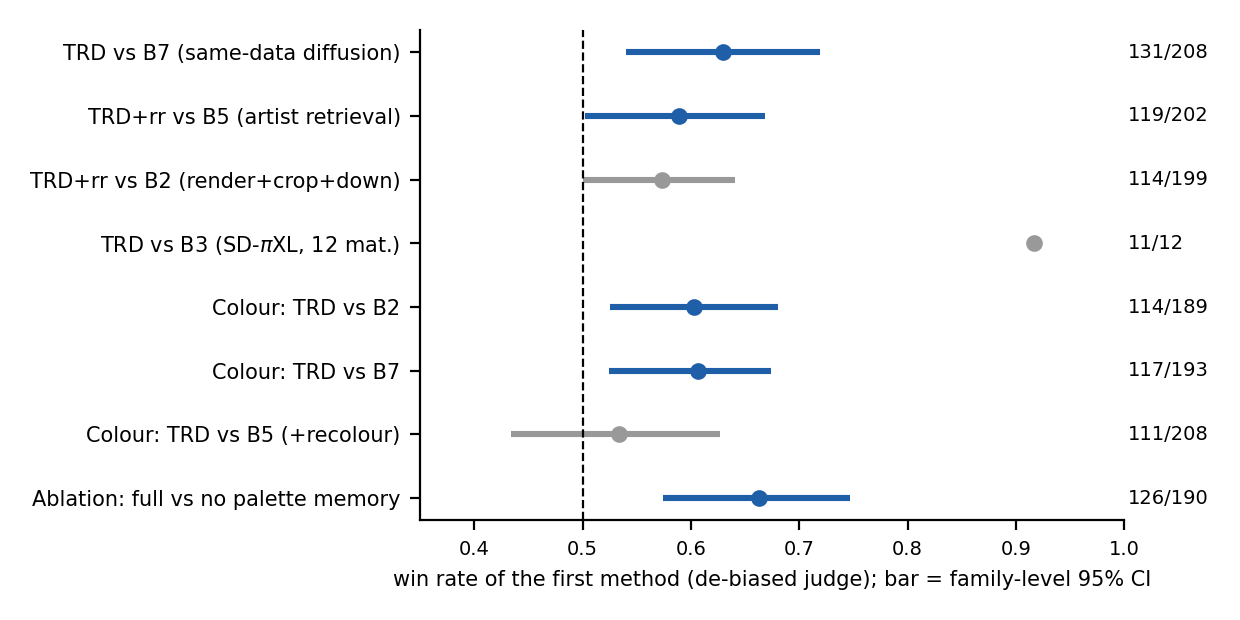
\includegraphics[width=0.74\linewidth]{../figures/fig_judge_forest.png}
\caption{All $16$px judge arms with family-level intervals. Blue: interval
excludes $0.5$. The SD-$\pi$XL arm ($n=12$) has only a binomial test. The last
row is the palette-memory ablation of \S\ref{sec:ablation}.}
\label{fig:forest}
\end{figure}

\subsection{The region-colouring task}

The full task paints a region of a given colour. Here every method receives the
target colour: \trd{} through its colour condition and colour-filtered
retrieval, the baselines through recolouring. To keep the comparison fair,
\emph{every} method, ours included, then receives the same Lab residual shift
that moves its mean colour onto the target. Table~\ref{tab:colour} shows that
the shift makes colour error negligible for all methods ($\Delta E\le0.32$),
so the comparison is about texture quality under a colour constraint. Natively,
without the shift, \trd{} already lands within $\Delta E=3.05$ of the target,
close to the just-noticeable range~\citep{sharma2005ciede2000}, whereas
recolouring the SDXL renders by palette mapping leaves $\Delta E\approx15$.
\trd{} has the best FID and CLIP score of all generators on this task, and the
judge prefers it over B2 ($60.3\%$) and B7 ($60.6\%$), both robust
(Table~\ref{tab:judge}). Against recoloured artist originals (B5), a
generator is being compared with the artists themselves; \trd{} holds its
own ($53.4\%$) while producing new tiles rather than copies.

\begin{table}[t]
\caption{Region-colouring task at $16$px ($857$ colour targets). ``+shift'':
the same Lab residual correction applied to every method. KID $\times10^3$.}
\label{tab:colour}
\centering
\small
\begin{tabular}{@{}lccccc@{}}
\toprule
Method & $\Delta E\downarrow$ & KID $\downarrow$ & FID $\downarrow$ & FD-DINOv2 $\downarrow$ & CLIP $\uparrow$ \\
\midrule
B1 + shift / palette recolour & 0.16 / 15.2 & 41.4 / 39.3 & 63.9 / 66.6 & 126.7 / 182.1 & 33.75 / 33.83 \\
B2 + shift / palette recolour & 0.17 / 15.3 & 24.6 / 26.9 & 55.1 / 58.6 & 151.2 / 179.5 & 34.21 / 34.08 \\
B7 + shift & 0.32 & \textbf{8.6} & 34.3 & \textbf{52.1} & 33.26 \\
\trd{} native / + shift & 3.05 / 0.30 & 10.2 / 9.9 & 31.4 / \textbf{31.2} & 53.5 / 54.2 & \textbf{34.30} / 34.29 \\
\midrule
\textcolor{gray}{B5 + shift (reference)} & \textcolor{gray}{0.23} & \textcolor{gray}{1.6} & \textcolor{gray}{29.7} & \textcolor{gray}{27.6} & \textcolor{gray}{33.68} \\
\bottomrule
\end{tabular}
\end{table}

\subsection{Ablations}
\label{sec:ablation}

All ablations are read against the noise floors of \S\ref{sec:protocol};
Table~\ref{tab:ablation} collects them.

\paragraph{Retrieval-augmented palettes carry the model.} Replacing the
retrieved palette by the model's own palette head raises KID from $9.7$ to
$35.1$ and FID from $44.2$ to $68.2$ and lowers CLIP by $0.76$ --- the only
ablation that clears all three floors --- and the judge prefers the full model
in $66.3\%$ of pairs ($p=8\times10^{-6}$, family CI $[0.57,0.75]$). An earlier
decomposition pointed the same way: with artist palettes substituted, \trd{}'s
structure alone reaches KID $4.5$ against an artist-versus-artist floor of
$3.8$, so the grid stream was already near artist level and the palette was
the bottleneck.

\paragraph{The periodic bias is what makes a position-free model work.} We
ablated the bias in three parameter-matched ways, each retrained for $12$k
steps from a common checkpoint with the same recipe and seed on the validation
materials: (A1) zero the grid--grid bias, leaving the model with no spatial
signal at all; (A2) replace the harmonic features of Eq.~\ref{eq:bias} by
non-periodic power features of identical dimension, a drop-in with exactly the
same parameter count; (A3) wrap at a wrong period ($1.3N$). Quality collapses
without the periodic form: KID rises from $8.4$ to $26.9$ without the bias and
to $15.9$ with the same-size non-periodic encoding, both far above the $4.76$
floor, while the wrong-period variant, still periodic, is indistinguishable
($7.3$). The periodic bias is what lets the model express ``a mortar line
every four rows'' without absolute coordinates, and it does so while keeping
the exact shift equivariance of \S\ref{sec:bias}. (A1's low seam deviation
reflects a structureless bag of tokens, not better tiling.) The remaining components --- exemplars (judge $49.7\%$),
choice temperature ($55.8\%$) and reranking ($\Delta$KID $2.3$) --- stay
within noise, so the gains come from the two design choices above.

\begin{table}[t]
\caption{Ablations at $16$px. Top: variants of \trd{}+rr on the test set
(KID $\times10^3$; judge = full model vs.\ variant). Bottom: toroidal-bias
arms retrained from a common checkpoint, validation materials ($125$); seam = median
per-material $|r-1|$, lower is closer to ideal. Floors: KID $4.76$, FID $6.0$,
CLIP $0.41$.}
\label{tab:ablation}
\centering
\small
\begin{tabular}{@{}lccccc@{}}
\toprule
Variant & KID & FID & CLIP & Seam & Judge (full wins) \\
\midrule
\trd{}+rr (full) & 9.7 & 44.2 & 35.19 & -- & -- \\
\;-- palette memory (generate palette) & 35.1 & 68.2 & 34.42 & -- & \textbf{126/190 = 66.3\%} \\
\;-- structural exemplars & 10.3 & 44.2 & 35.18 & -- & 87/175 = 49.7\% \\
\;choice temperature $20\to4.5$ & 10.8 & 44.8 & 35.09 & -- & 86/154 = 55.8\% \\
\;-- 4$\to$1 reranking & 12.0 & 44.9 & 34.66 & -- & -- \\
\midrule
C: toroidal harmonic bias (control) & 8.4 & -- & -- & 0.225 & -- \\
A1: bias zeroed & 26.9 & -- & -- & 0.093 & -- \\
A2: non-periodic features, same \#params & 15.9 & -- & -- & 0.148 & -- \\
A3: wrap at wrong period & 7.3 & -- & -- & 0.219 & -- \\
\bottomrule
\end{tabular}
\end{table}

\subsection{Other resolutions}
\label{sec:resolutions}

At $24$px, a size never seen in training (App.~\ref{app:res}), \trd{}+rr matches B2 ($50.0\%$) and beats B7 ($69.2\%$,
robust); at $32$px it beats B7 ($61.7\%$, robust) and SD-$\pi$XL ($10/12$).
All arms are listed in Appendix~\ref{app:res}.

% =====================================================================
\section{Conclusion}
\label{sec:limitations}

Pixel-art textures are small, discrete and toroidal, and \trd{} is built to
match. At $16$px it beats render pipelines on distribution metrics, is
preferred over same-data diffusion, artist retrieval and score distillation,
and wins the region-colouring task against the strongest pipeline and
same-data diffusion, with every claim checked against its noise floor. Each
advantage traces to a design choice: the palette--rank factorisation makes
colour a first-class input ($\Delta E=3.05$ natively versus $\approx15$ for
recoloured renders); the toroidal bias gives exact shift equivariance with
$6.5$k parameters, so no seam post-processing is needed; the palette memory
supplies the ramps a few thousand tiles cannot teach; and generating the tile
itself rather than a render to shrink makes it $28\times$ faster than the
strongest pipeline. None of the three components is tied to one engine or
to textures: they apply wherever images are small, palette-indexed or
periodic, from sprites and tile maps to textile patterns.

% =====================================================================
\section*{AI Use Statement}
Large language models were used as coding assistants for experiment scripts
and analysis code, to help draft and edit the text of this paper, and as the
pairwise judge described in \S\ref{sec:protocol}, whose selection and
protocol are reported there. All experimental designs, numbers and claims were
checked by the authors against the logged outputs.

\section*{Reproducibility Statement}
The dataset construction and split are described in \S\ref{sec:task}, the
architecture and training recipe in \S\ref{sec:method} and
Appendix~\ref{app:impl}, and the evaluation protocol, floors and judge
procedure in \S\ref{sec:protocol}. Code for training, sampling, all baselines,
metrics and the judge protocol, together with the per-arm judge outputs, will
be released with the paper.

\bibliography{refs}
\bibliographystyle{iclr2027_conference}

\appendix
\raggedbottom
\section{Implementation Details}
\label{app:impl}

\begin{table}[H]
\caption{\trd{} hyper-parameters (16px model).}
\label{tab:hparams}
\centering
\small
\begin{tabular}{@{}ll@{}}
\toprule
Backbone & 12 blocks, width 384, 6 heads, MLP ratio 4, dropout 0.1, adaLN-Zero \\
Parameters & 33M (bias module $\approx$6.5k) \\
Tokens & 16 palette slots (512-code colour codebook) + $N^2$ rank tokens \\
Toroidal bias & $F=8$ harmonics per axis, MLP hidden 128, shared across blocks \\
Text encoder & frozen CLIP ViT-B/32, prompt ``pixel art texture of \{name\}'' \\
Training & AdamW, lr $3\times10^{-4}$, wd 0.05, warm-up 1k, batch 256, 20k steps \\
Augmentation & uniform cyclic shift (all $N^2$ phases), horizontal flip \\
Masking & cosine schedule, palette and grid masked at the same ratio \\
Decoding & 24 steps, choice temperature 20, CFG 1.5, palette nucleus 0.9 \\
Retrieval & $n_\text{name}=30$ (100 for +rr), top-5, Lab mean shift \\
Reranking (+rr) & 4 samples, CLIP ViT-B/16 image--text similarity \\
\bottomrule
\end{tabular}
\end{table}

\paragraph{Judge prompt and bookkeeping.} Each pair is shown as two
nearest-neighbour enlargements of equal size, with the material name, and the
judge is asked which is the better pixel-art texture of that material. Every
pair is asked twice with positions swapped; API failures void an arm rather
than being dropped silently. Family intervals resample families of related
material names; an arm is additionally checked by leaving out one family at a
time, and arms with too few families (the SD-$\pi$XL subset) receive no family
interval.

\section{The Render-and-Downsample Baseline}

\begin{figure}[H]
\centering
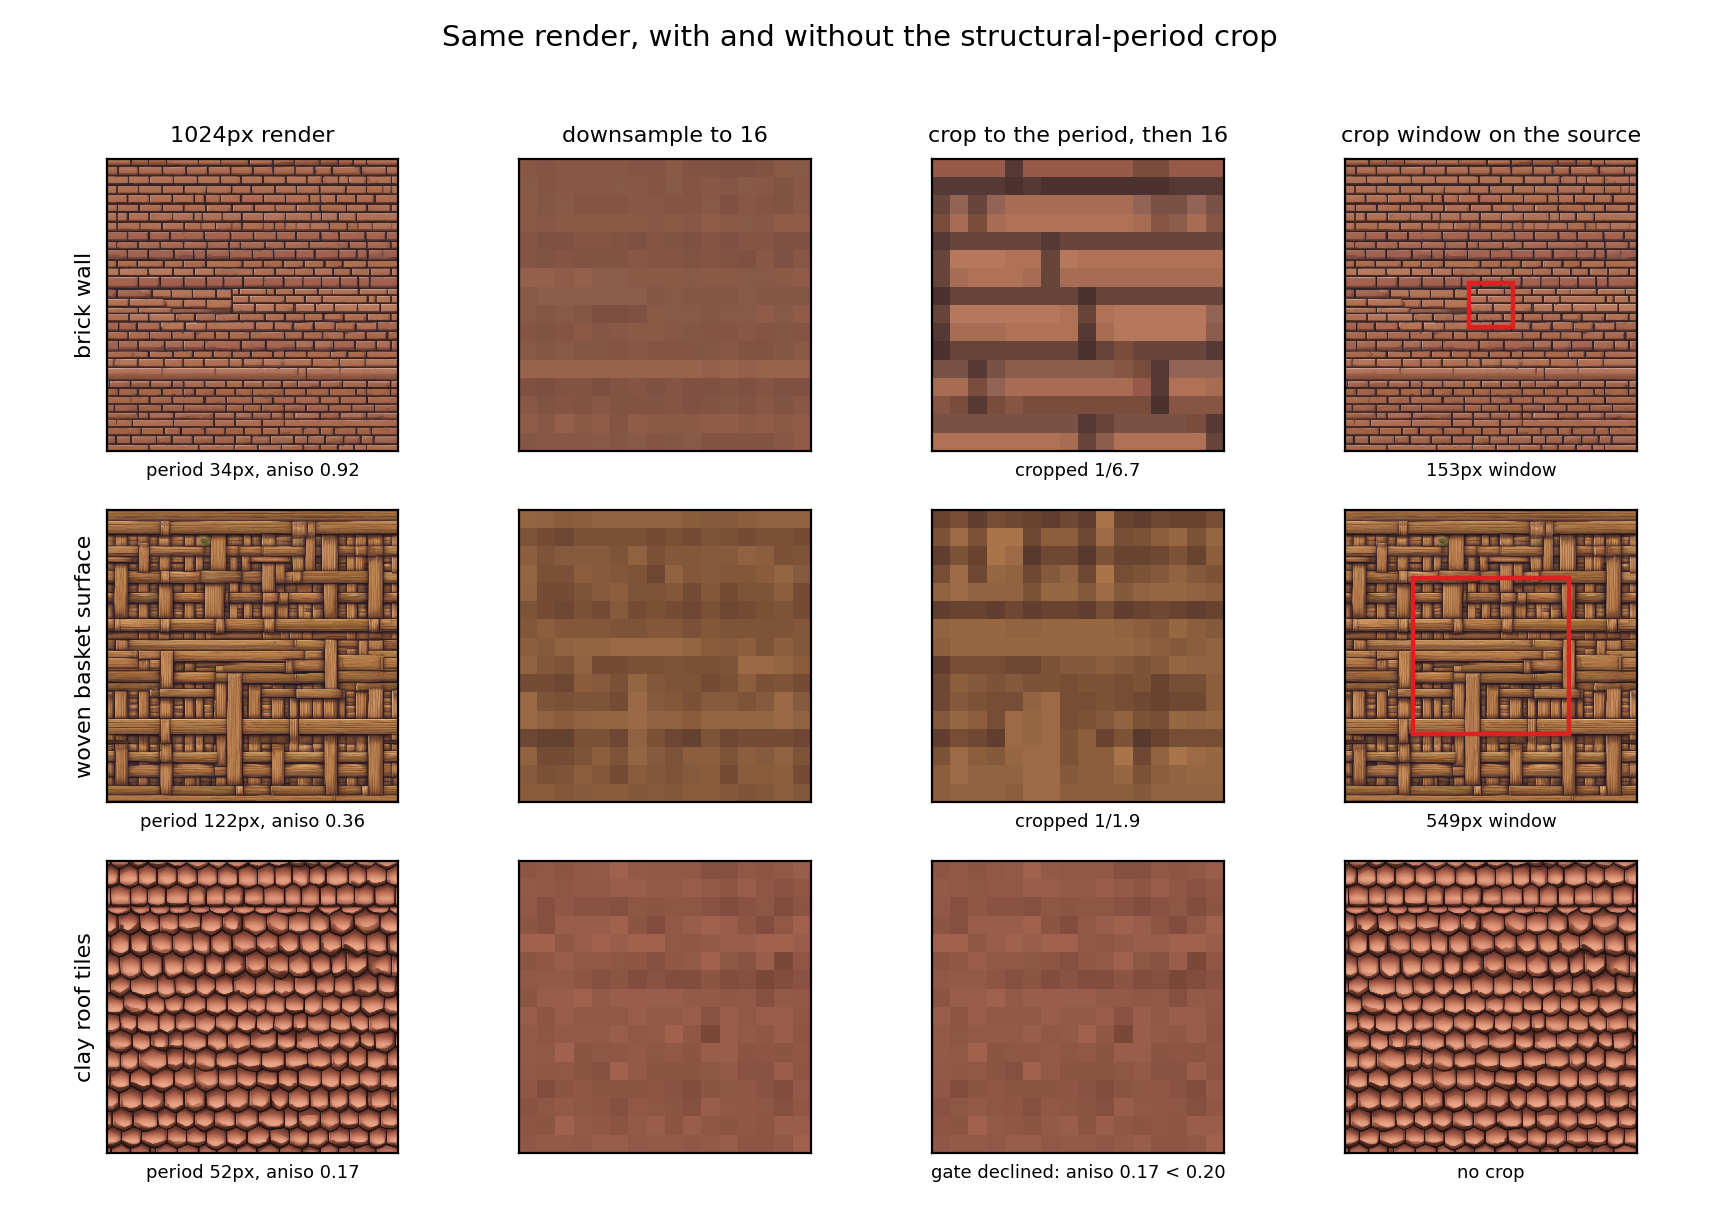
\includegraphics[width=0.92\linewidth]{../figures/fig_qualitative.png}
\caption{The strongest render-and-downsample baseline (B2). A $1024$px render
contains far more structural units than a $16$px tile can hold, so plain
downsampling (second column) loses the structure. Cropping to the detected
period first (third column) repairs it when a period exists; an anisotropy
gate declines to crop isotropic materials (bottom row). Because the crop is a
fixed multiple of the period, the same window yields more detail at a larger
target size --- the canvas gain of \S\ref{sec:protocol}.}
\label{fig:b2}
\end{figure}

\begin{figure}[H]
\centering
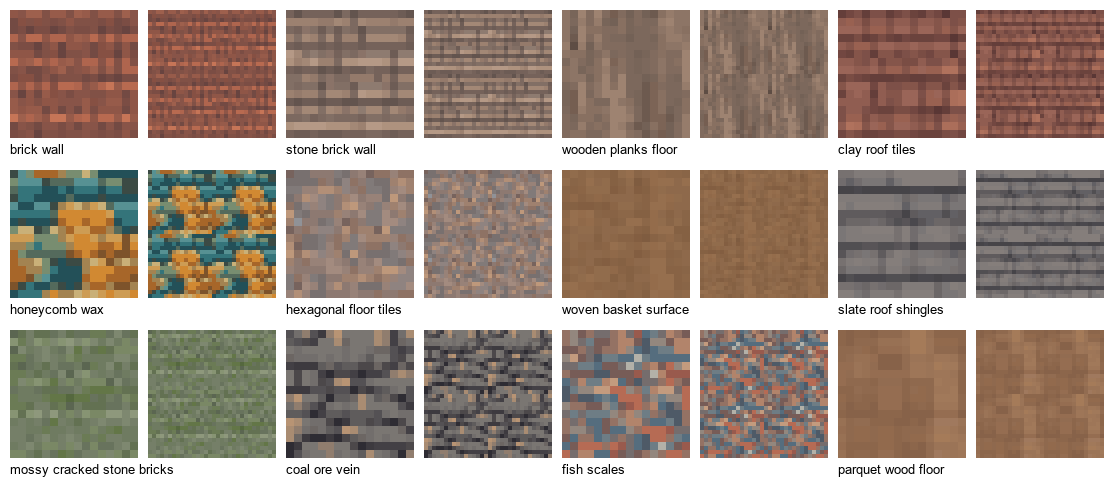
\includegraphics[width=\linewidth]{../figures/fig_supp_b2_gallery.png}
\caption{Best-of-4 outputs of the strongest baseline (B2, render + period crop
+ downsample) at $16$px for twelve generic material prompts
(not test-set materials; the test-set B2 samples are in Appendix~\ref{app:qual}). Each pair shows the tile
(left) and a $2\times2$ repetition (right), so seams and repeat artefacts are
visible. For strongly periodic materials (bricks, planks, roof tiles,
honeycomb) the crop yields clean, tileable structure, which is why B2 is the
strongest reference at this size (\S\ref{sec:experiments}); others, such as woven basket or parquet, lose most
of their structure at $16$px.}
\label{fig:b2gallery}
\end{figure}

\section{Additional Judge Arms and Results at 24 and 32px}
\label{app:res}

\begin{table}[H]
\caption{Additional judge arms on the test set: single-sample \trd{} at
$16$px, and all arms with CLIP scores at $24$ and $32$px (distribution metrics
are not reported there because the test packs contain too few artist tiles).}
\centering
\small\setlength{\tabcolsep}{4.5pt}
\begin{tabular}{@{}llcccc@{}}
\toprule
Size & Comparison & Wins / decided & Rate & $p$ & Family 95\% CI \\
\midrule
16 & \trd{} (single sample) vs B5 & 113 / 213 & 52.6\% & 0.41 & [0.447, 0.627] \\
16 & \trd{} (single sample) vs B2 & 90 / 190 & 47.4\% & 0.51 & [0.395, 0.553] \\
24 & \trd{}+rr vs B2 & 94 / 188 & 50.0\% & 1.0 & [0.421, 0.575] \\
24 & \trd{}+rr vs B7 & 144 / 208 & 69.2\% & $2.9\times10^{-8}$ & \textbf{[0.631, 0.753]} \\
32 & \trd{}+rr vs B7 & 116 / 188 & 61.7\% & 0.0016 & \textbf{[0.535, 0.698]} \\
32 & \trd{}+rr vs B1 & 105 / 186 & 56.5\% & 0.091 & [0.486, 0.642] \\
32 & \trd{}+rr vs B3 (12 mat.) & 10 / 12 & 83.3\% & 0.039 & n/a \\
32 & \trd{}+rr vs B2 & 83 / 202 & 41.1\% & 0.014 & [0.315, 0.502] \\
\midrule
\multicolumn{6}{@{}l}{CLIP at 24px: B1 35.17, B2 35.73, B4 \textbf{35.86}, B7 33.83, \trd{}+rr 35.66} \\
\multicolumn{6}{@{}l}{CLIP at 32px: B1 34.63, B2 \textbf{35.52}, B4 35.43, B7 33.73, \trd{}+rr 34.70} \\
\bottomrule
\end{tabular}
\end{table}

\begin{figure}[H]
\centering
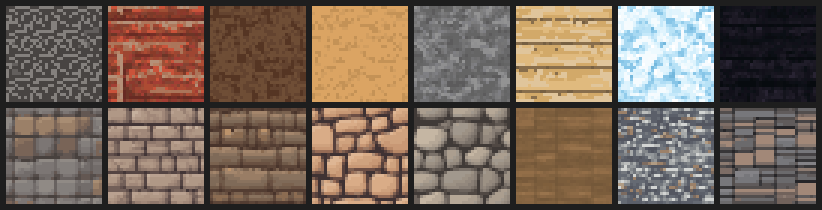
\includegraphics[width=\linewidth]{../experiments/sheet32_trd_vs_b2.png}
\caption{$32$px samples for eight materials, \trd{}+rr (top row) and B2
(bottom row), nearest-neighbour enlarged. The two families scale differently
with the canvas. B2 crops a fixed number of periods, so a larger canvas shows
the same block-level units with more cells (the canvas gain of Ruler~2).
\trd{} keeps the per-pixel density of authored $16$px art: its edge density at
$32$px relative to $16$px is $0.954$, against $0.840$ for B2 (paired
$p=4.2\times10^{-10}$).}
\label{fig:sheet32}
\end{figure}

\section{Qualitative Results at 16px}
\label{app:qual}

All samples below are the test-set outputs scored in \S\ref{sec:experiments}
(first sample per material; \trd{}+rr is the reranked sample). Every cell shows
a $2\times2$ repetition of the $16$px tile, nearest-neighbour enlarged, so
seams and repeat artefacts are visible. The artist tile is the held-out
reference for that material; no method saw it, and B5 retrieves from the
training split only. Figure~\ref{fig:qualcolour} covers the region-colouring
task and Figure~\ref{fig:qualname} the name-only task, whose panel (a) is
selected and panel (b) is not.

\begin{figure}[H]
\centering
\begin{minipage}[c]{0.42\linewidth}
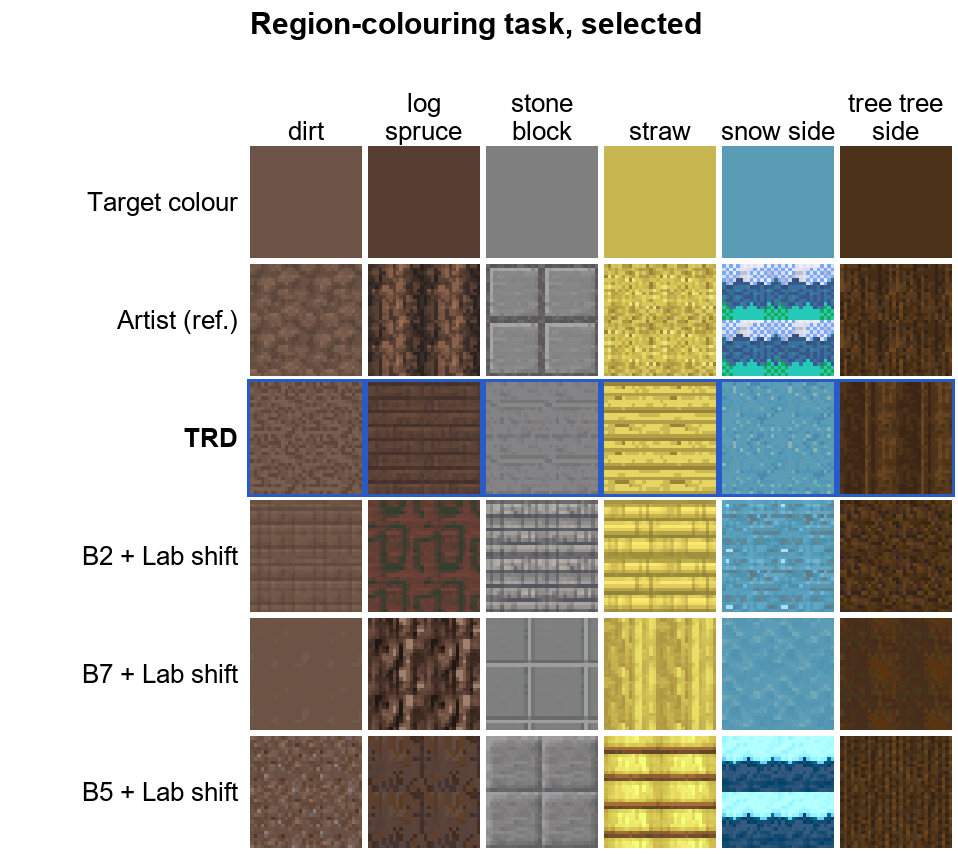
\includegraphics[width=\linewidth]{../figures/fig_supp_colour.png}
\end{minipage}\hfill
\begin{minipage}[c]{0.54\linewidth}
\caption{Region-colouring task, \emph{selected} from the 32 test materials on
which the judge preferred \trd{} over all three recoloured baselines. The
target is the artist tile's mean colour; baselines are Lab-shifted to it
afterwards (\trd{} gets the same shift as a residual correction), so
differences lie in structure and palette spread. \trd{} follows the target
natively with material-appropriate structure, whereas a post-hoc shift keeps
whatever the baseline drew, including structure foreign to the material (B2
on log spruce and stone block).}
\label{fig:qualcolour}
\end{minipage}
\end{figure}

\begin{figure}[H]
\centering
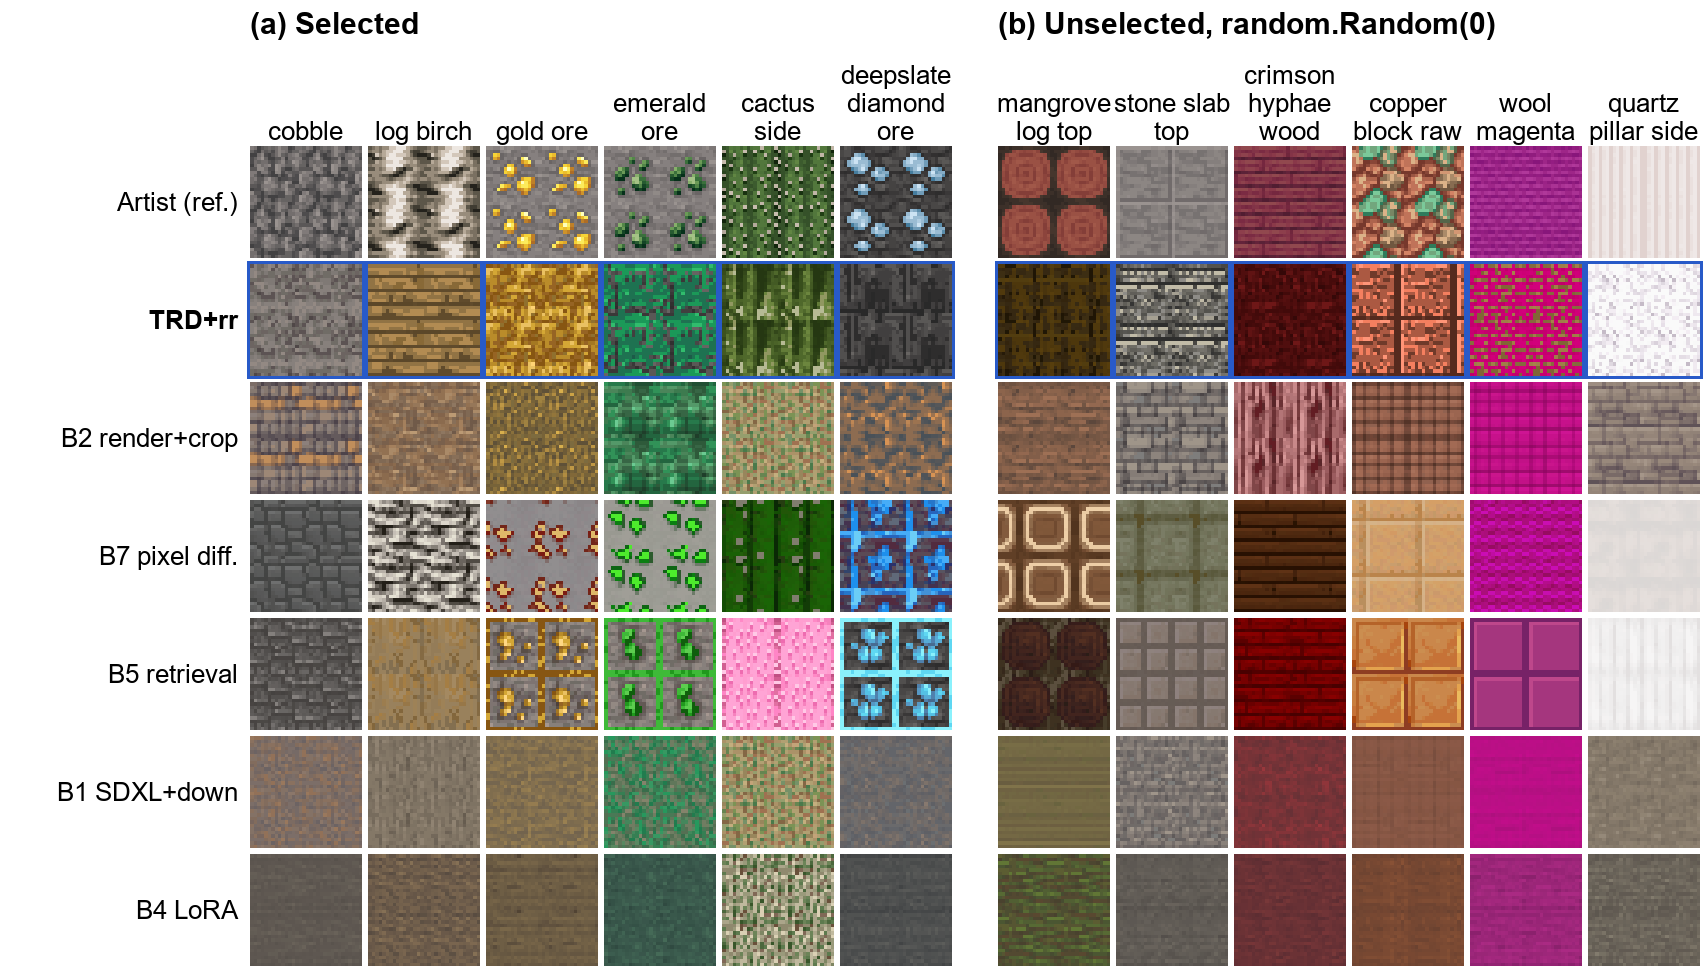
\includegraphics[width=\linewidth]{../figures/fig_supp_qual_name.png}
\caption{Name-only task; rows are methods, columns are test materials.
\textbf{(a) Selected:} chosen by us for variety from the 70 of 272 test
materials on which the judge preferred \trd{}+rr over both B2 and B5 (both
presentation orders agreeing). \trd{} keeps material-appropriate palettes and
repeats seamlessly, whereas B1 and B4 wash out to near-uniform fills and B2's
crop can pick the wrong structure (cobble, cactus side). \textbf{(b)
Unselected:} six of the 272 test materials drawn with a fixed seed
(\texttt{random.Random(0)}) before looking at the samples, shown so that
panel (a) can be read against typical outputs.}
\label{fig:qualname}
\end{figure}



\end{document}
